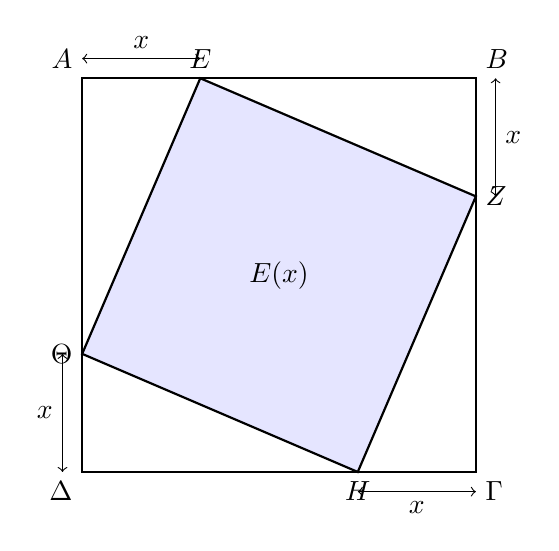
\begin{tikzpicture}[scale=0.5]
    % Coordinates of large square ABCD (side 10)
    \coordinate (A) at (0,10);
    \coordinate (B) at (10,10);
    \coordinate (C) at (10,0);
    \coordinate (D) at (0,0);

    % Draw ABCD
    \draw[thick] (A) -- (B) -- (C) -- (D) -- cycle;

    % Variable x
    \def\x{3} % Example value for x

    % Coordinates of inscribed square TH-H-Z-E
    \coordinate (E) at (\x,10);
    \coordinate (Z) at (10,10-\x);
    \coordinate (H) at (10-\x,0);
    \coordinate (TH) at (0,\x);

    % Draw inscribed square
    \draw[thick, fill=blue!10] (E) -- (Z) -- (H) -- (TH) -- cycle;

    % Labels for ABCD
    \node[above left] at (A) {$A$};
    \node[above right] at (B) {$B$};
    \node[below right] at (C) {$\Gamma$};
    \node[below left] at (D) {$\Delta$};

    % Labels for inner square
    \node[above] at (E) {$E$};
    \node[right] at (Z) {$Z$};
    \node[below] at (H) {$H$};
    \node[left] at (TH) {$\Theta$};

    % Labels for x
    \draw[<->] (0,10.5) -- (\x,10.5) node[midway, above] {$x$};
    \draw[<->] (10.5,10) -- (10.5,10-\x) node[midway, right] {$x$};
    \draw[<->] (10, -0.5) -- (10-\x, -0.5) node[midway, below] {$x$};
    \draw[<->] (-0.5, 0) -- (-0.5, \x) node[midway, left] {$x$};

    % Optional info
    \node at (5,5) {$E(x)$};

\end{tikzpicture}
